\documentclass[a4paper]{article}
\usepackage[utf8]{inputenc}
\usepackage[russian]{babel}
\usepackage{listings}
\usepackage[a4paper]{geometry}
\usepackage{indentfirst}
\usepackage{graphicx}
\usepackage{caption}
\usepackage{float}
\usepackage{amssymb}
\usepackage{physics}

\begin{document}

\title{Лабораторная работа 6 по курсу <<Нелинейная динамика и её приложения>>. \\Отчёт.}
\author{Владислав Соврасов\\ 381503м4}
\date{}
\maketitle

\section{Построение бифуркационной диаграммы логистичекого отображения}

\begin{figure}[H]
	\center
	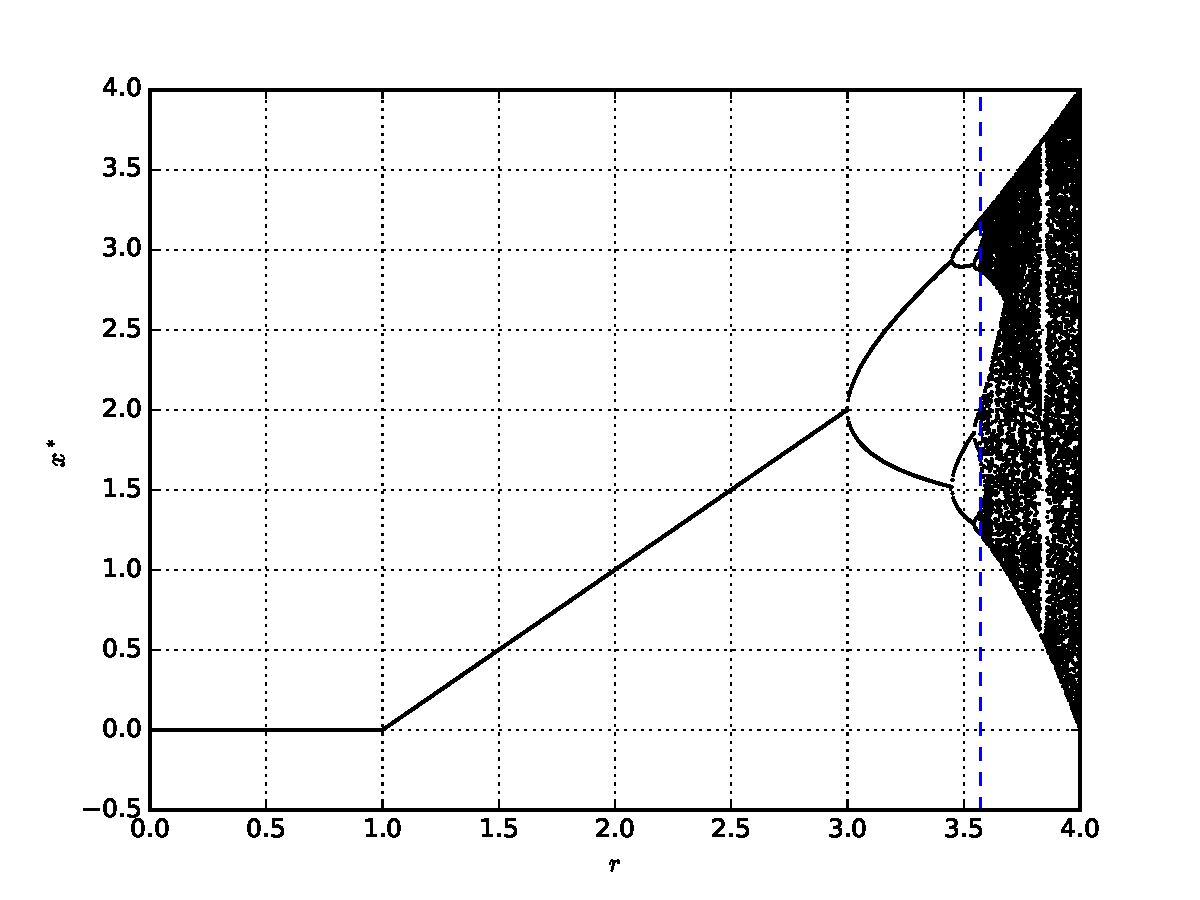
\includegraphics[width=0.75\textwidth]{../pictures/lab6_bifurcation_diagram.pdf}
	\caption{Бифуркационная диаграмма логистическго отображения}
	\label{fig:bifurcation_diagram}
\end{figure}

\section{Исследование устойчивости логистичекого отображения на аттракторе}

\begin{figure}[H]
	\center
	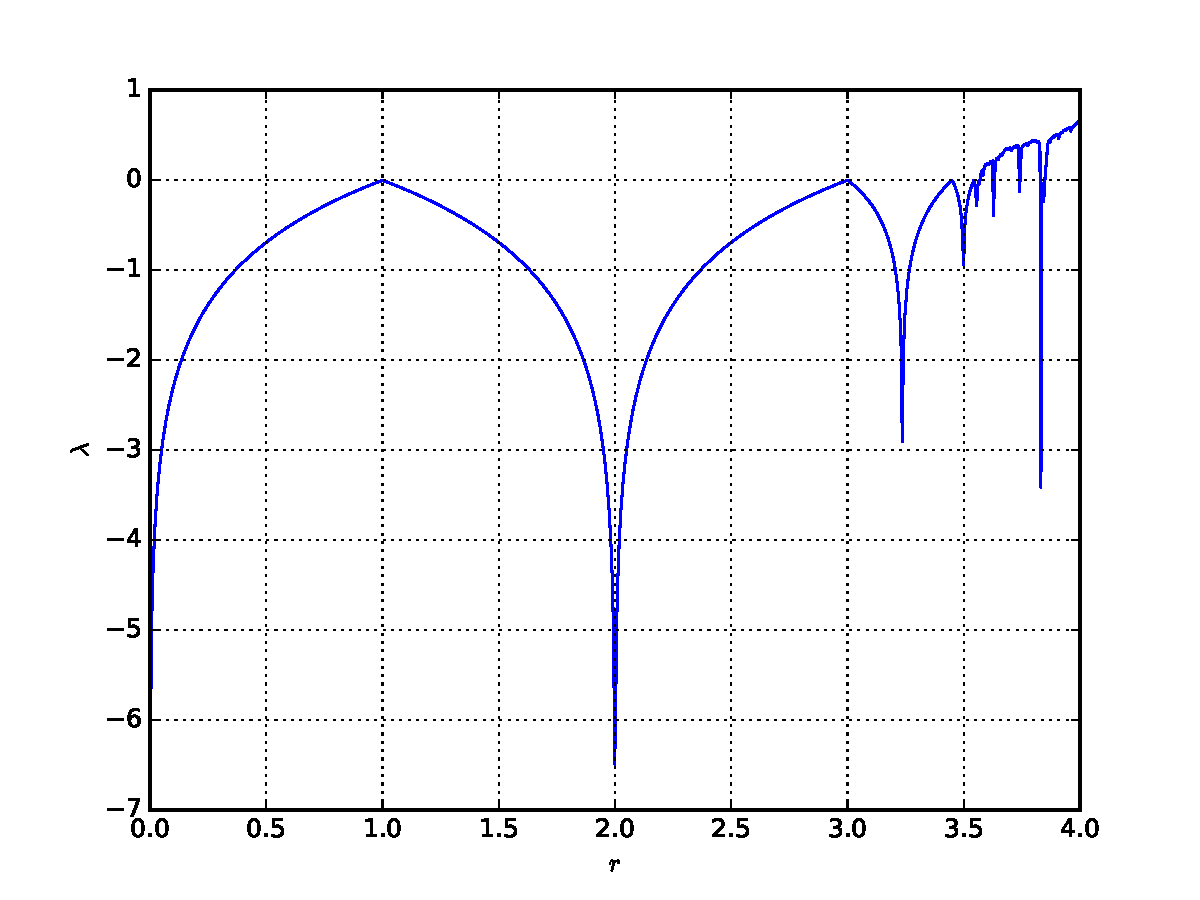
\includegraphics[width=0.75\textwidth]{../pictures/lab6_lyapunov_characteristic.pdf}
	\caption{Зависимость показателя Ляпунова от параметра отображения}
	\label{fig:lyapunov_characteristic}
\end{figure}

\section{Исходный код}
\lstinputlisting[language=Python, numbers=left]{../scripts/lab6.py}

\end{document}
